% SCIS Research Paper: PEG cylindrical multi-UAV pursuit under partial observability.
\documentclass{SCIS2026}

\begin{document}
\ArticleType{RESEARCH PAPER}
\Year{2026}
\Month{November}
\Vol{}
\No{}
\DOI{}
\ArtNo{}
\ReceiveDate{}
\ReviseDate{}
\AcceptDate{}
\OnlineDate{}
\AuthorMark{Anonymous authors}
\AuthorCitation{Anonymous authors}

\title[Multi-UAV pursuit among occluding cylinders]{Expert-guided learning for multi-UAV pursuit among occluding cylinders}{Expert-guided learning for multi-UAV pursuit among occluding cylinders}

\author[1]{Anonymous AUTHOR}{{corresponding.author@example.com}}
\address[1]{Affiliation withheld for anonymous review, City 000000, Country}

\abstract{Multi-UAV pursuit in cluttered free flight is challenging when vertical cylinders simultaneously constrain motion and interrupt onboard sensing of the target. This paper studies three pursuers that chase a scripted goal-seeking evader in a GPU-parallel PhysX environment with sixteen static cylinders and three moving obstacles. Capture is defined as three-dimensional swept body contact between the evader and any living pursuer, whereas the evader succeeds by reaching a northern goal ball without failure. Classical baselines are evaluated under a geometric MID-360 track that is occluded by cylinders. Separately, expert-guided MAPPO and MATD3 actors are evaluated under privileged ground-truth relative observations on the Medium speed band, with a shield or MPC teacher providing demonstrations and safety filtering. Under MID-360 sensing, a shield heuristic attains a capture rate of 0.62 on 50 stratified baseline episodes (horizontal evader-speed limit $2.0$~m/s). On a matched Medium-band ground-truth evaluation of 128 episodes, a frozen MAPPO clone reaches 0.59 against its shield teacher at 0.55, while a MATD3 run with EPN and AEG ends at a clone checkpoint of 0.46 without a completed online RL phase. The study clarifies the PEG contact-and-occlusion contract and separates MID-360 baseline metrics from ground-truth learner metrics. No real-flight performance is claimed.}

\keywords{cooperative pursuit--evasion, cylindrical occlusion, partial observability, multi-agent reinforcement learning, trajectory prediction, curriculum learning}
\maketitle

\section{Introduction}
Cooperative aerial pursuit--evasion couples continuous flight dynamics with intermittent sensing whenever obstacles interrupt line of sight~\cite{lavalle2006,bopardikar2008,zhou2016}. Classical geometric guidance and visibility-based formulations clarify how detection regions and cover constrain capture~\cite{gerkey2006,viper2025}, while recent deep multi-agent controllers explore online planning with motion prediction and adaptive curricula in unknown layouts~\cite{open2024,yu2022}. Many aerial studies, however, either assume privileged target state, planar kinematics, sparse urban prisms, or success criteria that do not match contact-based free-flight capture under dense vertical clutter.

We focus on a PEG-style free-flight arena in which static cylinders act as full-height collision columns and, under onboard sensing, also occlude target measurements. Three pursuers must contact a single evader that runs a goal-avoid policy toward a northern goal while dodging cylinders and pursuers. Relative to building-prism dual-capture protocols, the present task changes three contracts at once: obstacles are cylinders plus moving disks rather than a handful of urban prisms; success for the pursuers is single-vehicle swept contact rather than simultaneous two-of-three proximity; and difficulty is scheduled mainly by evader speed bands rather than a five-level joint change of buildings and sensor range.

The paper reports two complementary evaluation protocols on the same PhysX plant. Classical guidance baselines use a geometric MID-360 surrogate whose detections are gated by range, elevation, and cylinder occlusion, then filtered into per-pursuer tracks with teammate sharing. The archived learner comparisons instead use privileged ground-truth relative observations (including aim-point features) under Medium-band speeds, so that expert-guided cloning can be measured without conflating sensing dropouts. Expert guidance combines a shield or MPC teacher with offline-to-online constraints for MAPPO and MATD3, optionally with an LSTM evader prediction network (EPN) and a discrete adaptive environment generator (AEG). Weak-link outages and real-flight transfer are outside the present scope.

The contributions are threefold. First, we formalize a PEG observation and termination contract in which cylinders both block bodies and can hide MID-360 measurements. Second, we describe an expert-guided MAPPO/MATD3 pipeline with shield-style safety filtering and optional EPN/AEG modules, and we record the training settings that actually produced the reported checkpoints. Third, we report MID-360 classical baselines and Medium-band ground-truth learner evaluations as separate protocols, clarifying that they must not be pooled with historical dual-capture urban tables.

\section{Related work}
\subsection{Geometric and visibility-based pursuit}
Pursuit--evasion has a long geometric and game-theoretic lineage, from sensing-limited discrete-time formulations to cooperative Voronoi strategies~\cite{bopardikar2008,zhou2016,lavalle2006}. Visibility-based search emphasizes detection under restricted fields of view~\cite{gerkey2006}, and recent reinforcement learning variants treat visibility as an explicit objective~\cite{viper2025}. These lines clarify sensing constraints but do not by themselves specify three-dimensional contact capture among rigid aerial bodies navigating dense cylindrical clutter.

\subsection{Multi-agent learning for aerial cooperation}
Multi-agent reinforcement learning provides practical centralized-training, decentralized-execution recipes for cooperative control~\cite{yu2022}. Online multi-UAV pursuit in unknown environments has further combined deep policies with short-horizon prediction and adaptive environment generation~\cite{open2024}. Imitation and offline-to-online methods reduce exploration cost when a classical teacher is available, including DAgger-style relabeling and twin-critic actors with behavior cloning~\cite{ross2011,fujimoto2018,fujimoto2021}. Quadrotor simulation platforms such as OmniDrones enable GPU-parallel rigid-body learning under geometric tracking control~\cite{xu2024omnidrones,lee2010}.

\subsection{Positioning of this work}
The present study sits at the intersection of these threads, but adopts a PEG plant whose obstacles, capture event, and sensing occlusion differ from dual-capture urban prisms. We therefore treat prior five-level building tables as related context rather than as numerically pooled baselines, and we report PEG results under an explicit contact-and-occlusion contract. Table~\ref{tab:contract} summarizes the distinction that motivates the rewritten experimental protocol.

\begin{table}[H]
\footnotesize
\caption{Contract difference between a typical building-prism dual-capture setting and the PEG cylinder setting used in this paper.}
\label{tab:contract}
\begin{tabularx}{\textwidth}{Xcc}
\toprule
Item & Building-prism dual capture & PEG cylinder (this work) \\\hline
Static obstacles & Few urban prisms & 16 vertical cylinders \\
Dynamic obstacles & Often absent & 3 moving disks \\
Pursuer success & Two-of-three proximity ball & Any living pursuer contact \\
Typical capture radius & $\sim$1.0--1.5~m center ball & $\sim$0.6~m swept contact \\
Difficulty axis & Joint buildings/speed/sensing & Mainly evader speed bands \\
AEG levels & Often five profiles & Medium/Hard/Severe \\
Sensing occlusion & Prism faces & Cylinder disk--segment test (MID-360 protocol) \\
\bottomrule
\end{tabularx}
\end{table}

\section{Problem formulation}
\subsection{Arena, agents, and dynamics}
Figure~\ref{fig:scene} illustrates the arena used throughout this work. The horizontal workspace is approximately $\pm10.5\times\pm13.0$~m. Sixteen static cylinders are sampled with radii in $[0.2,0.55]$~m inside a clearance-constrained region; three dynamic obstacles move as planar disks with radii in $\{0.125,0.25,0.375,0.5\}$~m and speeds in $[0.5,1.5]$~m/s. Training and evaluation use free-3D flight with altitude roughly in $[0.5,14]$~m. Physics integrates at $\Delta t_{\rm phys}=0.02$~s; each policy decision lasts $\Delta t=0.2$~s (ten substeps). Pursuer horizontal, vertical, and yaw-rate limits are approximately $1.48$~m/s, $0.8$~m/s, and $1.4$~rad/s. Spawn uses PEG stratified sampling with start--goal clearance.

Let $p_{i,t}\in\mathbb{R}^3$ denote the position of pursuer $i$ at decision index $t$, and let $p^e_t$ denote the evader position. Cylinders are treated as vertical columns for collision: contact with an inflated cylinder is a failure that disables the contacting aircraft for the remainder of the episode. Aircraft cannot clear a cylinder by flying over it under the collision model. Dynamic obstacles and peer bodies use three-dimensional swept contact with the same body radius $r_{\rm body}$.

\begin{figure}[t]
\centering
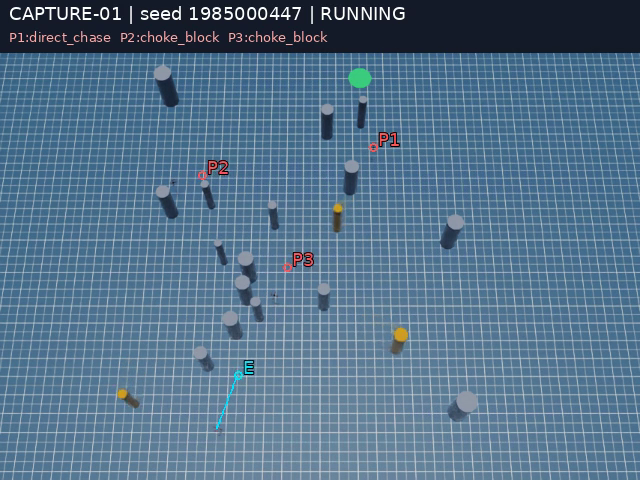
\includegraphics[width=0.98\textwidth]{figures/figure1_peg_cylinders.png}
\caption{PEG free-flight layout matching Section~\ref{sec:arena}. Gray vertical cylinders are static full-height collision columns; orange cylinders mark moving obstacles; P1--P3 are pursuers and E is the scripted evader heading toward the northern green goal. Contact with a cylinder terminates that aircraft as a failure. Under the MID-360 protocol, a cylinder of occlusion height $3$~m that intersects a pursuer--target segment also hides the measurement.}
\label{fig:scene}
\end{figure}

\subsection{Capture, goal, and termination}
\label{sec:arena}
Let $r_{\rm body}=0.3$~m. Between consecutive decision times, body centers follow piecewise-linear swept segments. A pursuer captures the evader when the minimum distance between the pursuer and evader swept segments is at most $2r_{\rm body}$:
\begin{equation}
\min_{\tau\in[0,1]}\bigl\|(p_{i,t}+\tau\Delta p_{i,t})-(p^e_t+\tau\Delta p^e_t)\bigr\|_2 \le 2r_{\rm body},
\label{eq:capture}
\end{equation}
which corresponds to approximately $0.6$~m contact. The evader succeeds if it enters a three-dimensional goal ball near the northern side without a concurrent failure. Termination priority follows capture, static collision, dynamic collision, out-of-bounds, physical failure, evader success, then timeout. Disabled pursuers no longer capture or collide; remaining living pursuers may continue.

\subsection{Scripted evader}
The evader is not co-learned. It follows a goal-avoid policy with vertical evasion that steers toward the goal while repelling from pursuers and cylinders. When discrete AEG is active, horizontal and vertical speed limits follow Table~\ref{tab:levels} (Medium uses $1.46$ and $0.84$~m/s). The MID-360 baseline matrix instead uses a horizontal speed limit of $2.0$~m/s with vertical evasion up to $0.88$~m/s. This scripted opponent provides a reproducible benchmark; it is not claimed to be a Nash-optimal evader.

\subsection{Observation--action interface}
A parameter-shared actor outputs
\begin{equation}
a_{i,t}=\bigl[(v^{\rm ref}_{i,t})^{\rm T},\dot\psi^{\rm ref}_{i,t}\bigr]^{\rm T},
\label{eq:action}
\end{equation}
where a normalized action in $[-1,1]$ is mapped to a world-frame velocity reference and a yaw-rate reference. A Lee-style position controller~\cite{lee2010} tracks these references on Hummingbird rigid bodies in Isaac Sim/PhysX~\cite{xu2024omnidrones}. GPU GridCloner parallelizes many PEG instances in one process.

Two observation interfaces appear in the reported experiments. Under the MID-360 protocol (Section~\ref{sec:mid360}), $o_{i,t}$ is built from filtered tracks and clearances. Under the ground-truth learner protocol used for Table~\ref{tab:peg-learner}, $o_{i,t}$ concatenates simulator relative positions and aim-point features, so the actor does read privileged target geometry at inference for those runs.

\section{Proposed method}
Figure~\ref{fig:system} summarizes the closed loop. Depending on the protocol, the actor consumes either MID-360 tracks or ground-truth relative features. An optional EPN appends short-horizon forecasts. The shared actor emits velocity and yaw-rate references; a shield or MPC teacher supplies demonstrations and safety filtering. Discrete AEG can re-select Medium/Hard/Severe evader speeds after finished episodes.

\begin{figure}[t]
\centering
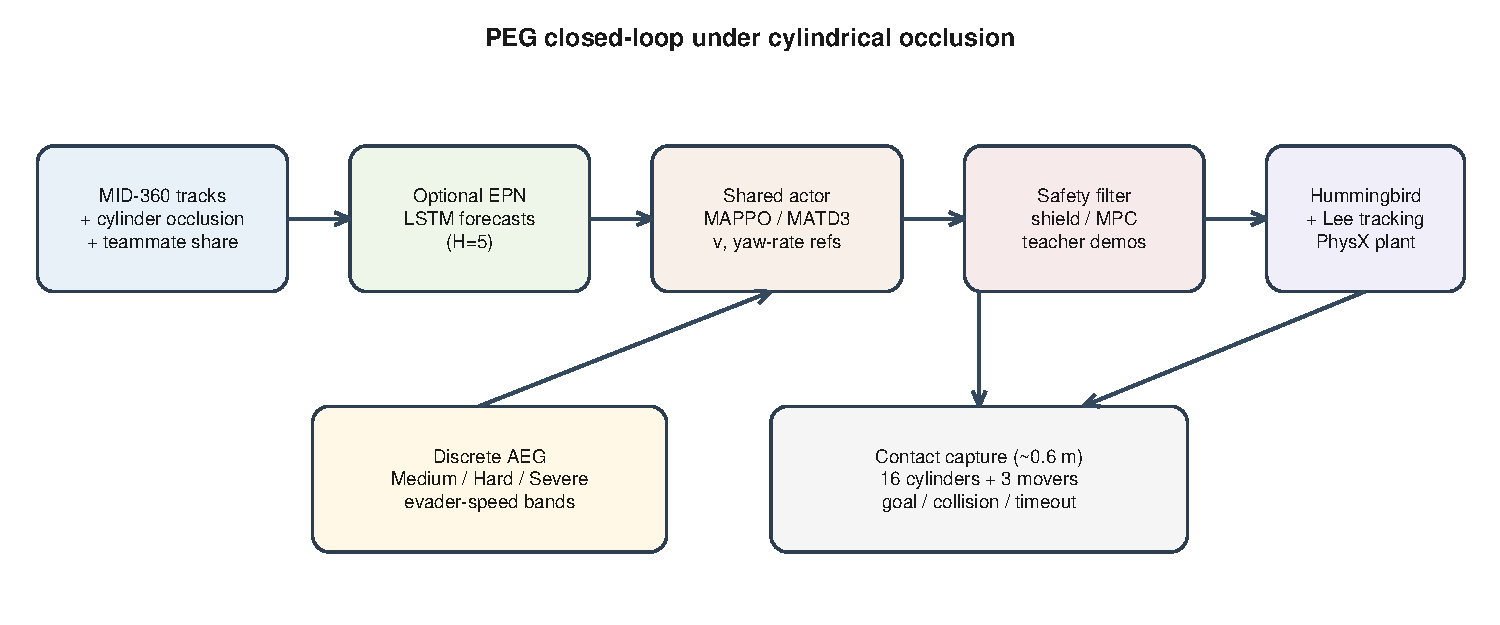
\includegraphics[width=0.98\textwidth,height=0.42\textheight,keepaspectratio]{figures/figure2_closed_loop_framework.pdf}
\caption{Closed loop under the PEG contract. The observation branch is protocol-dependent: MID-360 tracks with cylinder occlusion for classical baselines, or privileged ground-truth relative features for the archived learner comparisons. An optional EPN appends short-horizon forecasts. The shared actor outputs velocity and yaw-rate references for Hummingbird/Lee tracking. A shield or MPC teacher supplies demonstrations and safety filtering; MAPPO and MATD3 produce the reported checkpoints under the settings in Section~\ref{sec:exp}.}
\label{fig:system}
\end{figure}

\subsection{MID-360 sensing and tracks}
\label{sec:mid360}
The MID-360 protocol uses a geometric surrogate per pursuer~\cite{open2024}. Range is $[0.2,16]$~m, horizontal field of view is $360^\circ$, and elevation lies in $[-7^\circ,52^\circ]$. Detection probability is $0.88$ after the opening measurement. Additive position noise uses $0.08+0.005\,d$ meters for range $d$. A target is invisible if it fails the field-of-view test or if the pursuer--target segment intersects any static or dynamic cylinder of occlusion height $H_{\rm occ}=3$~m. Tracks smooth velocity with coefficient $\alpha=0.35$, coast for at most $0.8$~s, and drop after $2.5$~s without updates. Teammate odometry remains shared; only the evader is gated by MID-360. This protocol is used for the classical baseline matrix and is the intended deployable sensing interface; it is not the observation used by the archived MAPPO/MATD3 learner rows in Table~\ref{tab:peg-learner}.

\subsection{Reward design}
\label{sec:reward}
Two reward scales appear in the present codebase and runs. The default PEG reward used for the main training stack awards capture $+6$, collision $-20$, and a distance term with coefficient $0.1$ (normalized by a $10$~m scale), with discount $\gamma=0.995$. The archived Table~\ref{tab:peg-learner} training runs instead used a denser terminal scale of capture $+100$ and collision $-30$. Evaluation metrics remain capture, goal, timeout, and collision rates and do not depend on which training scale was used.

\subsection{Classical teachers}
The primary classical teacher for recent PEG runs is a shield heuristic: lead pursuit composed with half-space braking against cylinders, moving obstacles, walls, and peers. Let $v^{\rm lead}$ denote a lead-pursuit velocity toward a predicted intercept, and let $\{n_k\}$ denote outward normals of active half-spaces. The shield projects
\begin{equation}
v^{\rm sh}=\Pi_{\{v:\,v^{\rm T}n_k\ge b_k\}}(v^{\rm lead}),
\label{eq:shield}
\end{equation}
where $b_k$ encodes a safety margin and braking strength. MPC variants sample discrete velocity candidates and reject those whose swept bodies collide before issuing references. Demonstrations from these teachers initialize actors. Shield is preferred as a cloning teacher not because it always tops the MID-360 capture ranking, but because its commanded actions stay closer to the aim-point geometry that the learner imitates.

\subsection{Expert-guided MAPPO}
For on-policy learning, MAPPO~\cite{yu2022} maximizes a clipped surrogate while sharing parameters across pursuers. Expert guidance enters through demonstration regression and a KL regularizer. Let $\pi_\theta$ be the current actor and $\pi_{\rm ref}$ a frozen imitation reference. The implemented KL term compares the current actor to the frozen reference:
\begin{equation}
\mathcal{L}_{\rm MAPPO}=\mathcal{L}_{\rm PPO}(\theta)+\lambda_{\rm dem}\,\mathbb{E}\bigl[\|a_\theta-a^{\rm dem}\|_2^2\bigr]+\lambda_{\rm KL}\,D_{\rm KL}\bigl(\pi_\theta\,\|\,\pi_{\rm ref}\bigr).
\label{eq:mappo}
\end{equation}
For the archived Medium ground-truth MAPPO clone that yields capture rate $0.59$, the imitation/clone weight remained at $1$ throughout and was not annealed toward a smaller floor. At evaluation, the learner action excludes teacher mixing while retaining the safety shield.

\subsection{Expert-guided MATD3}
For off-policy learning, MATD3 follows a twin-critic recipe with behavior cloning and an actor objective of the form
\begin{equation}
\mathcal{L}_{\rm act}=-\mathbb{E}\bigl[Q_{\phi_1}(o,\pi_\theta(o))\bigr]+\lambda_{\rm BC}\,\mathbb{E}\bigl[\|\pi_\theta(o)-a^{\rm dem}\|_2^2\bigr]+\lambda_{\rm anc}\,\mathbb{E}\bigl[\|\pi_\theta(o)-\pi_{\rm anc}(o)\|_2^2\bigr].
\label{eq:matd3}
\end{equation}
For the archived MATD3 checkpoint reported at capture rate $0.46$, EPN and AEG were enabled, but the online actor RL phase did not successfully start; the evaluated weights are the clone checkpoint retained at the end of that run. The replay buffer for that run did not drop transitions from failed episodes, and the actor anchor was not kept as a frozen reference for the reported result. Evaluation uses the actor mean without teacher mixing in the executed command.

\subsection{Evader prediction network}
\label{sec:epn}
Following prediction-enhanced partial-observability designs~\cite{open2024}, an LSTM EPN maps a length-$L=10$ causal history to $H_{\rm fut}=5$ future relative positions. Privileged future evader poses supervise mean-squared-error training only:
\begin{equation}
\mathcal{L}_{\rm EPN}=\frac{1}{H_{\rm fut}}\sum_{k=1}^{H_{\rm fut}}\bigl\|\hat\delta_{t+k}-\delta^{\star}_{t+k}\bigr\|_2^2.
\label{eq:epn}
\end{equation}
EPN is optional. It is enabled in the archived MATD3 run and is intended primarily to help under intermittent MID-360 tracks; its incremental contribution still requires matched ablations.

\subsection{Discrete adaptive environment generator}
\label{sec:aeg}
Discrete AEG selects among Medium, Hard, and Severe after each finished episode using a rolling capture window of length $W=50$: undersampled levels first; then levels with empirical capture rate in $[0.5,0.9]$; otherwise bias harder or easier when the global rate falls outside that band~\cite{open2024}. Cold start defaults to Hard (or Medium in some launches). Evader speed limits are listed in Table~\ref{tab:levels}. The Medium learner evaluation freezes Medium speeds; AEG was enabled during the archived MATD3 training run but is not claimed as an evaluated module for the MAPPO clone row.

\begin{table}[H]
\footnotesize
\caption{Evader-speed bands used by discrete AEG. Values are horizontal and vertical speed limits in m/s.}
\label{tab:levels}
\begin{tabularx}{\textwidth}{lcc}
\toprule
Level & Horizontal & Vertical \\\hline
Medium & 1.46 & 0.84 \\
Hard & 1.52 & 0.88 \\
Severe & 1.72 & 1.00 \\
\bottomrule
\end{tabularx}
\end{table}

\section{Experiments}
\label{sec:exp}
\subsection{Protocol}
All experiments share the PEG cylinder plant (sixteen static cylinders, three dynamic obstacles, free-3D, swept contact). Two protocols are reported separately.

\paragraph{MID-360 classical baselines.}
Table~\ref{tab:peg-baselines} uses 50 stratified seeds from 1000 with MID-360 sensing. The scripted evader uses goal-avoid with vertical evasion up to $0.88$~m/s and horizontal speed limit $2.0$~m/s, which is not the AEG Medium band ($1.46/0.84$~m/s).

\paragraph{Ground-truth Medium learner evaluation.}
Table~\ref{tab:peg-learner} uses 128 matched Medium-band episodes. Actors consume privileged ground-truth relative observations with aim-point features, not MID-360 tracks. Capture rate is primary; goal, timeout, and collision rates are auxiliary. Heterogeneous-graph variants, unfinished DAgger curricula, and layout-curriculum experiments without completed evaluation are excluded from these tables.

\subsection{Classical guidance under MID-360 occlusion}
Table~\ref{tab:peg-baselines} reports APF, FRPN, discrete-candidate MPC, and the shield heuristic under identical MID-360 baseline seeds (34/50, 13/50, 16/50, and 31/50 captures, respectively). APF reaches the highest capture rate (0.68). Shield reaches 0.62 and is retained as the cloning teacher because its actions align more closely with aim-point intercepts that learners imitate, not because it dominates APF on capture rate. MPC and FRPN capture less often (0.32 and 0.26) while conceding more goals. Track-valid fractions are reported as secondary sensing statistics; a low track-valid rate (e.g., APF at 0.35) should not be read as ``no estimate for $65\%$ of time'' without an explicit missing-estimate counter, and a high track-valid rate (FRPN at 0.79) does not imply high capture.

\begin{table}[H]
\footnotesize
\caption{PEG baselines under MID-360 sensing (50 episodes; 16 cylinders + 3 dynamic obstacles; free-3D). Evader horizontal limit $2.0$~m/s (not AEG Medium). Capture: any living pursuer contacts the evader. Goal: evader reaches the northern goal ball without failure.}
\label{tab:peg-baselines}
\begin{tabularx}{\textwidth}{Xcccc}
\toprule
Method & Capture & Goal & Timeout & Track valid \\\hline
APF & 0.68 & 0.12 & 0.08 & 0.35 \\
FRPN & 0.26 & 0.62 & 0.00 & 0.79 \\
MPC & 0.32 & 0.14 & 0.32 & 0.57 \\
Shield & 0.62 & 0.12 & 0.10 & 0.40 \\
\bottomrule
\end{tabularx}
\end{table}

\subsection{Expert-guided actors under ground-truth Medium observations}
Table~\ref{tab:peg-learner} compares frozen learners to the matched shield teacher on Medium-band evaluation with ground-truth observations (128 episodes; speeds $1.46/0.84$~m/s). The learner executes the actor mean with safety shield on and no teacher mixing in the action.

The MAPPO clone reaches capture rate $0.59$ ($76/128$) versus the shield teacher at $0.55$ ($70/128$), with goals $3/128$ versus $33/128$, timeouts $18$ versus $1$, and collision rates $0.234$ versus $0.188$. Actor inputs are concatenated ground-truth relative features including aim points. This row is therefore not a MID-360 result.

The MATD3 run with EPN and AEG reaches capture rate $0.46$ ($59/128$) from the clone weights retained at the end of training; the online RL phase did not complete for that archive. It does not exceed the matched shield teacher under this protocol. Hard/Severe transfers and controlled EPN/AEG ablations remain future work.

\begin{table}[H]
\footnotesize
\caption{Medium-band PEG evaluation under ground-truth observations (128 episodes; speeds $1.46/0.84$~m/s). Not MID-360. Learner control: actor mean, safety shield on, no teacher mixing. MAPPO: accepted clone. MATD3: clone checkpoint after a run with EPN/AEG in which online RL did not start.}
\label{tab:peg-learner}
\begin{tabularx}{\textwidth}{Xcccc}
\toprule
Method & Capture & Goal & Timeout & Collision \\\hline
Shield teacher & 0.55 & 0.26 & 0.01 & 0.19 \\
MAPPO (clone, GT obs.) & 0.59 & 0.02 & 0.14 & 0.23 \\
MATD3 clone (EPN+AEG run) & 0.46 & 0.15 & 0.17 & 0.20 \\
\bottomrule
\end{tabularx}
\end{table}

\subsection{Difficulty scheduling and metric boundaries}
Discrete AEG operates on three evader-speed bands (Table~\ref{tab:levels}). Absolute rates from the MID-360 baseline matrix (horizontal limit $2.0$~m/s) must not be ranked against Medium ground-truth learner rates, and neither should be pooled with historical building-prism dual-capture tables.

\subsection{Failure modes and qualitative observations}
Inspection of failed PEG episodes suggests three recurring patterns. First, aggressive line pursuit after a long coast can drive a pursuer into a cylinder. Second, peer repulsion and cylinder brakes in a shared corridor can cancel useful chase components and produce timeouts. Third, under MID-360, a brief occlusion window can leave tracks coasting while the evader reaches the northern goal. These observations motivate tighter shields and, for the sensing protocol, prediction under dropout, but they remain qualitative until episode-level logs are aggregated.

\subsection{Analysis and limitations}
Under MID-360 occlusion, classical line-of-sight guidance is brittle relative to shield/APF. Under privileged Medium observations, a MAPPO clone can slightly exceed its shield teacher on capture rate while reducing goal leakage, at the cost of more collisions and timeouts. The MATD3 archive reported here is a clone endpoint without a completed RL phase and should not be read as a finished off-policy learner.

All conclusions are bounded by the PEG plant: cylinders are full-height collision columns (MID-360 occlusion height $3$~m), capture is swept contact with body radius $0.3$~m, and the $5$~Hz velocity/yaw-rate interface does not claim SITL or real-flight rates. Communication is fully connected. The evader is scripted. Deployable MID-360 learning results are not claimed by Table~\ref{tab:peg-learner}.

\section{Conclusion}
This paper formulated multi-UAV pursuit among occluding cylinders as a PEG contact-and-occlusion contract with swept-body capture and three-band AEG. Classical MID-360 baselines and Medium-band ground-truth learner evaluations were reported as separate protocols. Under ground-truth Medium observations, a frozen MAPPO clone slightly exceeds its shield teacher on capture rate ($0.59$ vs.\ $0.55$) while reducing goal leakage, with higher collision rate ($0.23$ vs.\ $0.19$) and more timeouts ($18$ vs.\ $1$). Future work will complete MID-360 learner evaluations, matched EPN/AEG ablations, Hard/Severe transfers, and tighter safety filtering before any claim of real-flight readiness.

\Acknowledgements{To be completed before submission. The PEG parallel environment and training entry points used in this study are maintained in the configurable-pursuit codebase, with algorithm modules adapted from the cooperative aerial pursuit stack at \url{https://github.com/kuangyinying039/uav-swarm}. Isaac Sim and OmniDrones remain external dependencies~\cite{xu2024omnidrones}.}

\begin{thebibliography}{99}

\bibitem{lavalle2006} LaValle S M. Planning Algorithms. Cambridge: Cambridge University Press, 2006

\bibitem{bopardikar2008} Bopardikar S D, Bullo F, Hespanha J P. On discrete-time pursuit-evasion games with sensing limitations. IEEE Trans Robot, 2008, 24: 1429--1439

\bibitem{zhou2016} Zhou Z, Zhang W, Ding J, et al. Cooperative pursuit with Voronoi partitions. Automatica, 2016, 72: 64--72

\bibitem{gerkey2006} Gerkey B P, Thrun S, Gordon G. Visibility-based pursuit-evasion with limited field of view. Int J Robot Res, 2006, 25: 299--315

\bibitem{viper2025} Wang Y, Cao Y, Chiun J, et al. ViPER: visibility-based pursuit-evasion via reinforcement learning. In: Proceedings of the 8th Conference on Robot Learning, PMLR, 2025, 270: 4188--4200

\bibitem{yu2022} Yu C, Velu A, Vinitsky E, et al. The surprising effectiveness of PPO in cooperative multi-agent games. In: Advances in Neural Information Processing Systems, 2022, 35: 24611--24624

\bibitem{open2024} Zhang R, Xu J, Yu C, et al. Online planning for multi-UAV pursuit-evasion in unknown environments using deep reinforcement learning. arXiv:2409.15866, 2024

\bibitem{ross2011} Ross S, Gordon G, Bagnell D. A reduction of imitation learning and structured prediction to no-regret online learning. In: Proceedings of the Fourteenth International Conference on Artificial Intelligence and Statistics, 2011. 627--635

\bibitem{fujimoto2018} Fujimoto S, van Hoof H, Meger D. Addressing function approximation error in actor-critic methods. In: Proceedings of the 35th International Conference on Machine Learning, 2018. 1587--1596

\bibitem{xu2024omnidrones} Xu B, Gao F, Yu C, et al. OmniDrones: an efficient and flexible platform for reinforcement learning in drone control. IEEE Robot Autom Lett, 2024, 9: 2838--2844

\bibitem{lee2010} Lee T, Leok M, McClamroch N H. Geometric tracking control of a quadrotor UAV on SE(3). In: Proceedings of the 49th IEEE Conference on Decision and Control, 2010. 5420--5425

\bibitem{fujimoto2021} Fujimoto S, Gu S S. A minimalist approach to offline reinforcement learning. In: Advances in Neural Information Processing Systems, 2021, 34: 12678--12690

\end{thebibliography}

\end{document}
